\section{Anhang}
\subsection{Volumenkörper}

\hspace*{\fill}
\begin{minipage}[c]{0.2\columnwidth}
	$\mathbf{V} = l \cdot b \cdot h$
\end{minipage} 
\hfill
\begin{minipage}[c]{0.5\columnwidth}
	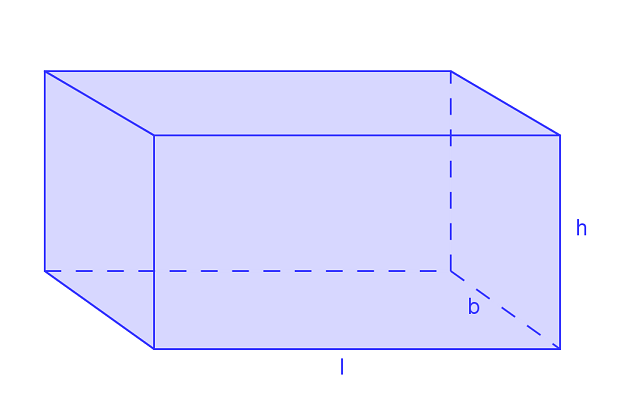
\includegraphics[scale=0.2]{koerper/Rechteck.png}
\end{minipage}
\hspace*{\fill}

\smallskip

\hspace*{\fill}
\begin{minipage}[c]{0.2\columnwidth}
	$\mathbf{V} = G \cdot h$
\end{minipage} 
\hfill
\begin{minipage}[c]{0.5\columnwidth}
	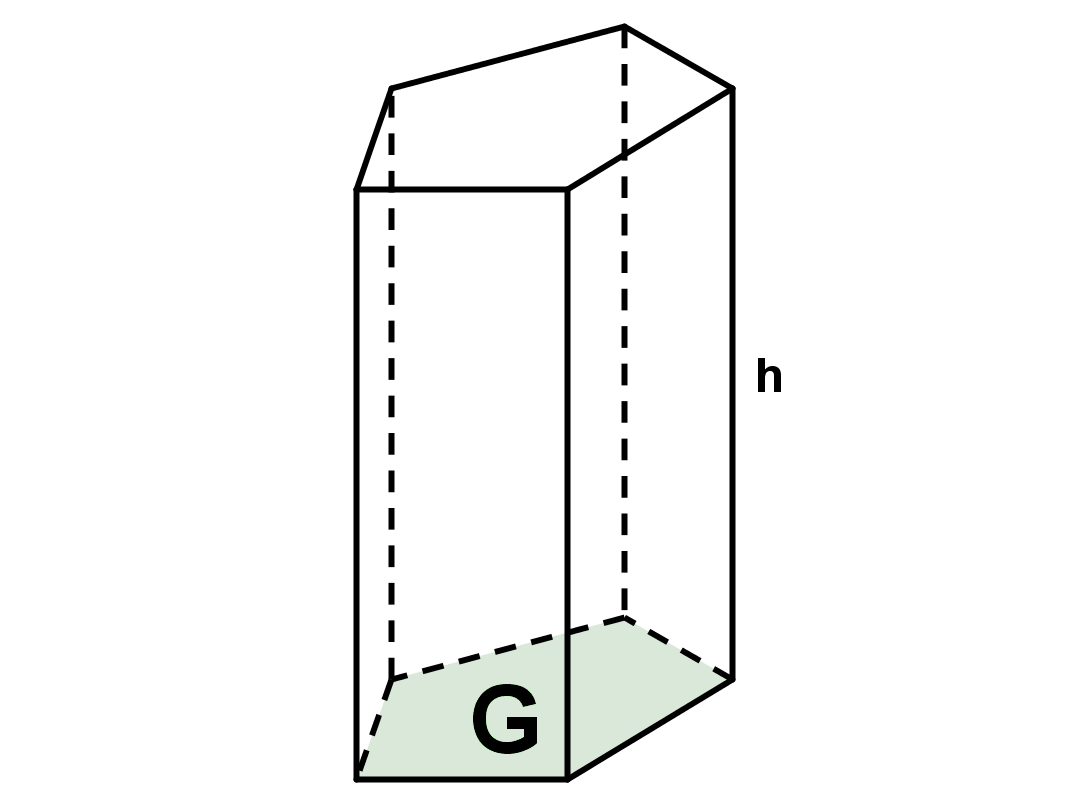
\includegraphics[scale=0.4]{koerper/Prisma.png}
\end{minipage}
\hspace*{\fill}

\smallskip

\hspace*{\fill}
\begin{minipage}[c]{0.2\columnwidth}
	$\mathbf{V} = r^2 \cdot \pi \cdot h $
\end{minipage} 
\hfill
\begin{minipage}[c]{0.5\columnwidth}
	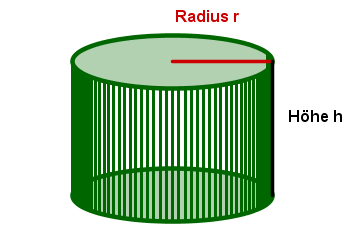
\includegraphics[scale=0.3]{koerper/Zylinder.png}
\end{minipage}
\hspace*{\fill}

\smallskip

\hspace*{\fill}
\begin{minipage}[c]{0.2\columnwidth}
	$\mathbf{V} = \frac{4\pi}{3} \cdot r^3$
\end{minipage} 
\hfill
\begin{minipage}[c]{0.5\columnwidth}
	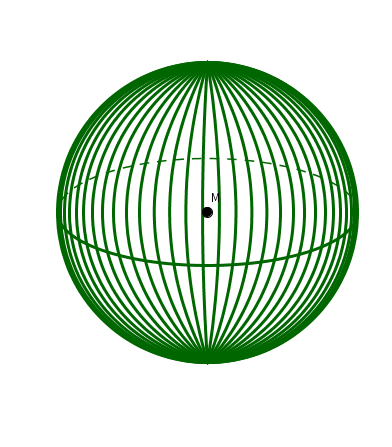
\includegraphics[scale=0.25]{koerper/Kugel.png}
\end{minipage}
\hspace*{\fill}

\smallskip

\hspace*{\fill}
\begin{minipage}[c]{0.2\columnwidth}
	$\mathbf{V} = \frac{1}{3} \cdot r^2 \cdot \pi \cdot h$
\end{minipage} 
\hfill
\begin{minipage}[c]{0.5\columnwidth}
	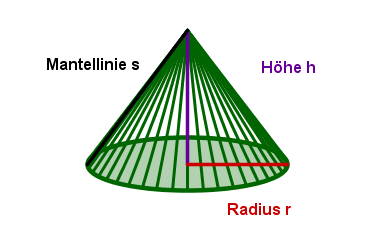
\includegraphics[scale=0.3]{koerper/Kegel.png}
\end{minipage}
\hspace*{\fill}

\smallskip

\hspace*{\fill}
\begin{minipage}[c]{0.2\columnwidth}
	$\mathbf{V} = a^3$
\end{minipage} 
\hfill
\begin{minipage}[c]{0.5\columnwidth}
	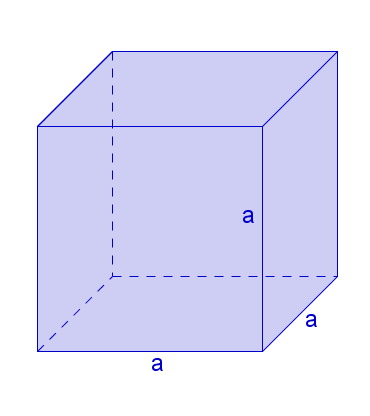
\includegraphics[scale=0.25]{koerper/Quader.png}
\end{minipage}
\hspace*{\fill}

\smallskip

\hspace*{\fill}
\begin{minipage}[c]{0.2\columnwidth}
	$\mathbf{V} =\frac{a^3}{12} \cdot \sqrt{2}$
\end{minipage} 
\hfill
\begin{minipage}[c]{0.5\columnwidth}
	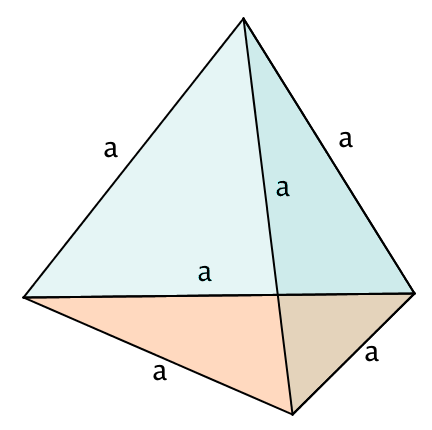
\includegraphics[scale=0.2]{koerper/Tetraeder.png}
\end{minipage}
\hspace*{\fill}

\subsection{Präfixe}
\begin{center}
	\begin{minipage}{0.5\columnwidth}
		\centering
		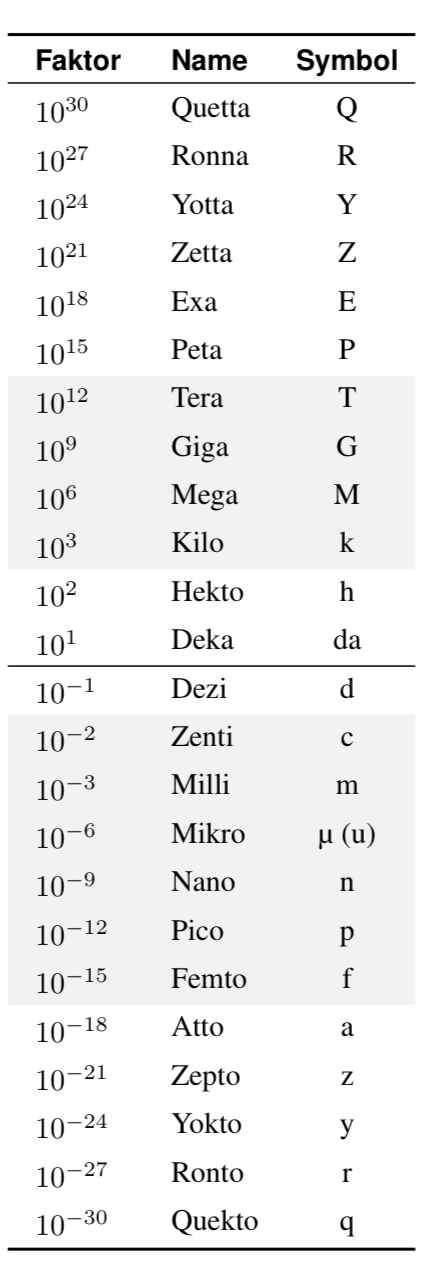
\includegraphics[width=0.6\columnwidth]{images/Praefixe.jpeg}
	\end{minipage}
\end{center}

\subsection{Molmassen wichtiger Atome}

\renewcommand{\arraystretch}{1.3}
\begin{tabular}{c | c | c }
	\textbf{Symbol} & \textbf{Molekül}  & \textbf{Molmasse}                 \\
	\hline
	H               & Wasserstoff       & $1.008 \, \frac{\gram}{\mole}$    \\
	C               & Kohlenstoff       & $12.011 \, \frac{\gram}{\mole}$   \\
	N               & Stickstoff        & $14.007 \, \frac{\gram}{\mole}$   \\
	O               & Sauerstoff        & $15.999 \, \frac{\gram}{\mole}$   \\
	Al              & Aluminium         & $26.982 \, \frac{\gram}{\mole}$   \\
	Si              & Silicium          & $28.982 \, \frac{\gram}{\mole}$   \\
\end{tabular}
\renewcommand{\arraystretch}{1.3}

\subsection{Weitere Einheiten von Druck}

\vspace{-0.2cm}
$$ \bm{1 \, \bbar = 10^5 \pascal} \qquad \text{Absolutdruck: Vergleich zu Vakuum} $$

\begin{tabular}{ll}
	$1 \, \hecto \pascal$   & $= 100 \, \pascal = 1 \, \milli \bbar $                                       \\
	$1 \, \mathrm{at}$      & $= 1 \, \mathrm{kp \cdot \centi \meter^{-2}} = 9.81 \cdot 10^4 \, \pascal$    \\
	$1 \, \mathrm{at"u}$    & $= 1 \, \mathrm{at}$ (Überdruck; Vergleich zu normalem Luftdruck)             \\
	$1 \, \mathrm{Torr}$    & $= \frac{1}{760} \, \mathrm{at}$ (1 mm-Hg-Säule)
\end{tabular}

\subsection{Wichtige Dichten}	

\begin{tabular}{l c l}
	$\rho_{\rm Wasser} = 1000 \, \frac{\kilogram}{\meter^3}$    & &  $\rho_{\rm Luft} = 1.2 \, \frac{\kilogram}{\meter^3}$
	
\end{tabular}

\subsection{Eigenschaften der Aggregatszustände}

\subsubsection{Festkörper}

\begin{itemize}
	\item Kein Fluid
	\item Festes Volumen; feste Gestalt
	\item Moleküle / Atome befinden sich in regelmässiger Gitter-Anordnung
	\item Inkompressibel (sehr schlecht komprimierbar)
	\item Kraft: Weiterleitung (längs ihrer Wirkungslinie)
	\item Druck: Verstärkung 
\end{itemize}


\subsubsection{Ideale Flüssigkeit}

\begin{itemize}
	\item Fluid
	\item Festes Volumen; keine feste Gestalt
	\item Moleküle / Atome bewegen sich chaotisch aneinander vorbei
	\item Moleküle / Atome füllen den Raum aus / berühren sich
	\item Inkompressibel (schlecht komprimierbar)
	\item Reibungsfrei (keine Scherkräfte)
	\item Kraft: Verstärkung
	\item Druck: Weiterleitung (gleichmässig)
\end{itemize}


\subsubsection{Gas}

\begin{itemize}
	\item Fluid
	\item Kein festes Volumen; keine feste Gestalt
	\item Moleküle / Atome fliegen mit hoher Geschwindigkeit durch den Raum
	\item Es gibt sehr viel Zwischenraum 
	\item Moleküle / Atome führen bei Zusammenstoss unter sich oder mit Gefässwand elestische Stösse aus
	\item Kompressibel (gut komprimierbar)
	\item Reibungsfrei (keine Scherkräfte)
\end{itemize}

\subsection{Hydrostatik ideale Fluide}

\subsubsection{Auftrieb}
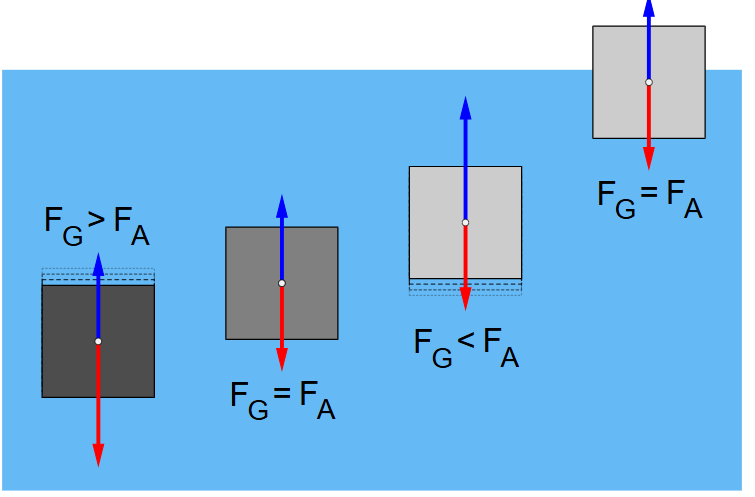
\includegraphics[width=0.8\columnwidth]{images/Auftrieb_3arten.png}
\break
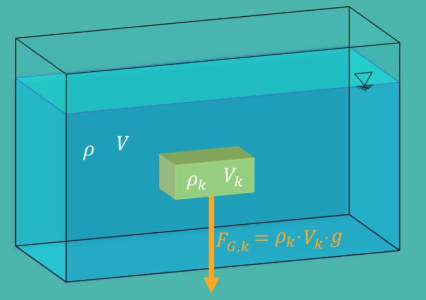
\includegraphics[width=0.7\columnwidth]{images/Auftrieb_3D.png}
\break
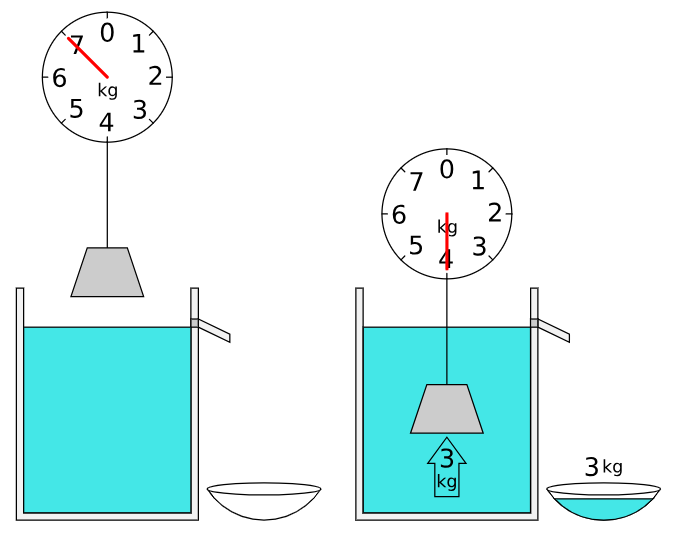
\includegraphics[width=0.7\columnwidth]{images/Kraefte_Auftrieb.png}

\subsubsection{Stromlinien-Modell}
\textbf{Ideale Fluide nehmen keine Scherkräfte auf (keine Reibung) und sind inkompressibel.}

\begin{itemize}
	\item Stromlinien zeigen Geschwindigkeit des Fluids
	\item \textbf{Dichte} Stromlinien bedeutet \textbf{hohe} Geschwindigkeit
	\item \textbf{Dünne} Stromlinien bedeutet \textbf{niedrige} Geschwindigkeit 
	\item Stationär: Stromlinien schneiden sich nicht 
\end{itemize}

\subsection{Hydrostatik reale Fluide}
\subsubsection{Helmholz'sche Wirbelsätze}

\begin{enumerate}
	\item Wirbel hat kein Anfang und kein Ende
	\item Wirbel besteht immer aus denselben Fluidteilchen
	\item Zirkulation zeitlich konstant
\end{enumerate}

\subsubsection[Druckwiderstand]{Druckwiderstand $\bm{F_D}$}\label{subsec:aerodynamik}

Beschreibt die turbulente Luftreibungskraft $F_R$ und wird meist als Luftwiderstand bezeichnet.

$$ \boxed{ F_D = \Delta \, p \cdot A_s = \frac{1}{2} \, \cdot \rho \cdot v^2 \cdot A_s \cdot c_W } $$

\renewcommand{\arraystretch}{1.3}
\begin{tabular}{c l c}
	$F_D$           & Druckwiderstand                           & $[F_D] = \newton$                     \\
	$\Delta \, p$   & Druckdifferenz                            & $[\Delta \, p] = \pascal$             \\
	$\rho$          & Luft-Dichte                               & $[\rho] = \frac{\kilogram}{\meter^3}$ \\
	$c_W$           & Widerstandsbeiwert / Widerstandszahl      & $[c_W] = 1$                           \\
	$v$             & Strömungs-Geschwindigkeit                 & $[v] = \frac{\meter}{\second}$        \\
	$A_s$           & Projizierte Fläche senkrecht zur Strömung & $[A_s] = \meter$
\end{tabular}
\renewcommand{\arraystretch}{1}

\medskip

\textrightarrow\ Der Widerstandsbeiwert $c_W$ ist \textbf{geometrieabhängig}!


\subsubsection[Auftriebskraft nach Kutta-Jukowski]{Auftriebskraft $\bm{F_A}$ nach Kutta-Jukowski}

Beschreibt die Proportionalität zwischen dynamischem Auftrieb und Zirkulation.

$$ \boxed{ F_A = \rho \cdot v \cdot l \cdot \Gamma } $$

\renewcommand{\arraystretch}{1.3}
\begin{tabular}{c l c}
	$F_A$       & Dynamischer Auftrieb      & $[F_A] = \newton$                     \\
	$\rho$      & Dichte des Fluids         & $[\rho] = \frac{\kilogram}{\meter^3}$ \\
	$v$         & Geschwindigkeit           & $[v] = \frac{\meter}{\second}$        \\
	$l$         & Länge quer zur Strömung   & $[l] = \meter$                        \\
	$\Gamma$    & Zirkulation               & $[\Gamma] = \frac{\meter^2}{\second}$
\end{tabular}
\renewcommand{\arraystretch}{1}


\subsubsection{Zirkulation $\bm{\Gamma}$}

Die Zirkulation ist ein Mass für die \textbf{Rotation} im Strömungsfeld

$$ \boxed{ \Gamma = \oint \vec{v} \bullet \diff \vec{s} } $$

\renewcommand{\arraystretch}{1.5}
\begin{tabular}{c l c}
	$\Gamma$                        & Zirkulation                       & $[\Gamma] = \frac{\meter^2}{\second}$     \\
	$\vec{v} \bullet \iff \vec{s}$  & Geschwindigkeit entlang dem Weg   & $[\vec{v}] = \frac{\meter}{\second}$      \\
	& Skalarprodukt: $\vec{v} \bullet  \diff \vec{s} = a \cdot b \cdot \cos(\varphi)$
\end{tabular}
\renewcommand{\arraystretch}{1}


\subsubsection[Dynamischer Auftrieb]{Dynamischer Auftrieb $\bm{F_A}$}

\vspace{-0.2cm}

$$ \boxed{ F_A = c_A \cdot \underbrace{\frac{1}{2} \cdot \rho \cdot v^2 }_{\substack{\Delta \, p}} \cdot A_{\|}	} $$

\renewcommand{\arraystretch}{1.3}
\begin{tabular}{c l c}
	$F_A$       & Dynamischer Auftrieb                              & $[F_A] = \newton$                     \\
	$c_A$       & Auftriebskoeffizient                              & $[c_A] = 1$                           \\
	$\rho$      & Luft-Dichte                                       & $[\rho] = \frac{\kilogram}{\meter^3}$ \\
	$v$         & Strömungsgeschwindigkeit                          & $[v] = \frac{\meter}{\second}$        \\
	$A_{\|}$    & Projizierte Fläche \textbf{parallel} zur Strömung & $[A_{\|}] = \meter^2$
\end{tabular}
\renewcommand{\arraystretch}{1}


\subsubsection{Wissenswertes zum dynamischen Auftrieb}

\begin{itemize}
	\item Ein gerade ausgerichtetes, symmetrisches Stromlinienprofil erzeugt \textbf{keinen} dynamischen Auftrieb
	\item An einem asymmetrischen Flügelprofil entsteht dynamischer Auftrieb 
\end{itemize}


\subsubsection[Induzierter Widerstand]{Induzierter Widerstand $\bm{F_W}$}

Kommt durch Energieverlust (Wirbelbildung) zu Stande, welcher entsteht, wenn die Umgebungsluft in Bewegung gesetzt wird.

$$ \boxed{ F_W = c^*_W \cdot \frac{1}{2} \cdot \rho \cdot v^2 \cdot A_{\|} } $$


\begin{tabular}{c l c}
	$F_W$       & Induzierter Widerstand                            & $[F_W] = \newton$                     \\
	$\rho$      & Luft-Dichte                                       & $[\rho] = \frac{\kilogram}{\meter^3}$ \\
	$c^*_W$     & Widerstands-Koeffizient                           & $[c*_W] = 1$                          \\
	$v$         & Strömungsgeschwindigkeit                          & $[v] = frac{\meter}{\second}$         \\
	$A_{\|}$    & Projizierte Fläche \textbf{parallel} zur Strömung & $[A_{\|}] = \meter^2$
\end{tabular}

\subsubsection[Gleitwinkel]{Gleitwinkel $\bm{\varphi}$}

Gibt die zurückgelegte Stecke pro verbrauchte Höhe an. Im Luft-Kanal ist dies der Anstell-Winkel.

$$ \boxed{ \tan(\varphi) = \frac{F_W}{F_A} = \frac{c^*_W}{c_A}= \frac{v_V}{v_H} } $$

\renewcommand{\arraystretch}{1.3}
\begin{tabular}{c l c}
	$\varphi$   & Gleitwinkel                   & $[\varphi] = \degree$             \\
	$F_W$       & Widerstandskraft              & $[F_W] = \newton$                 \\
	$F_A$       & Auftriebskraft                & $[F_A] = \newton$                 \\ 
	$c^*_W$     & Widerstands-Koeffizient       & $[c^*_W] = 1$                     \\
	$c_A$       & Auftriebs-Koeffizient         & $[c_A] = 1$                       \\
	$v_V$       & Vertikal-Geschwindigkeit      & $[v_V] = \frac{\meter}{\second}$  \\
	$v_H$       & Horizontal-Geschwindigkeit    & $[v_H] = \frac{\meter}{\second}$
\end{tabular}
\renewcommand{\arraystretch}{1}



\subsection{ideale Gase}

\subsubsection{Modell des idealen Gases}

\textbf{Jedes Gas ist gleich!}

\medskip

\begin{enumerate}
	\item Moleküle sind Massepunkte (keine Ausdehnung)
	\item Stösse sind elastisch (keine zwischenmolekularen Kräfte) \\
	Kein Volumen bei $T = 0$ \\
	Kein Druck bei $T = 0$
\end{enumerate}

\subsubsection{Zustandsgrössen}
\begin{tabular} {ll}
	Thermodynamische Systeme werden durch Zustandsgrössen beschrieben &  \\
	T, p, V, n, U, S & \\
\end{tabular}

\subsubsection{Doulong-Petit}

\text{Die 6 Freiheitsgrade eines einzelnen Kupferatoms im Festkörper sind also:}
\newline
\[
\underbrace{3 \text{ für die kinetische Energie}}_{\text{Schwingung in x, y, z}} + \underbrace{3 \text{ für die potentielle Energie}}_{\text{Auslenkung in x, y, z}} = 6 \text{ Freiheitsgrade}
\]
\newline
Weil jedes Atom in einem einfachen Festkörper (wie Kupfer) diese 6 Freiheitsgrade hat \\ (im Metallgitter sich in 3 Achsen bewegt und dadurch kinetische \\ wie auch potentielle energie hat), sagt das Äquipartitionsgesetz \\ eine molare Wärmekapazität von $c_M \approx 3R$ voraus, was experimentell sehr gut bestätigt wird.

\subsubsection{Tabelle ideale Gase und Wärmekapazität}

\begin{center}
	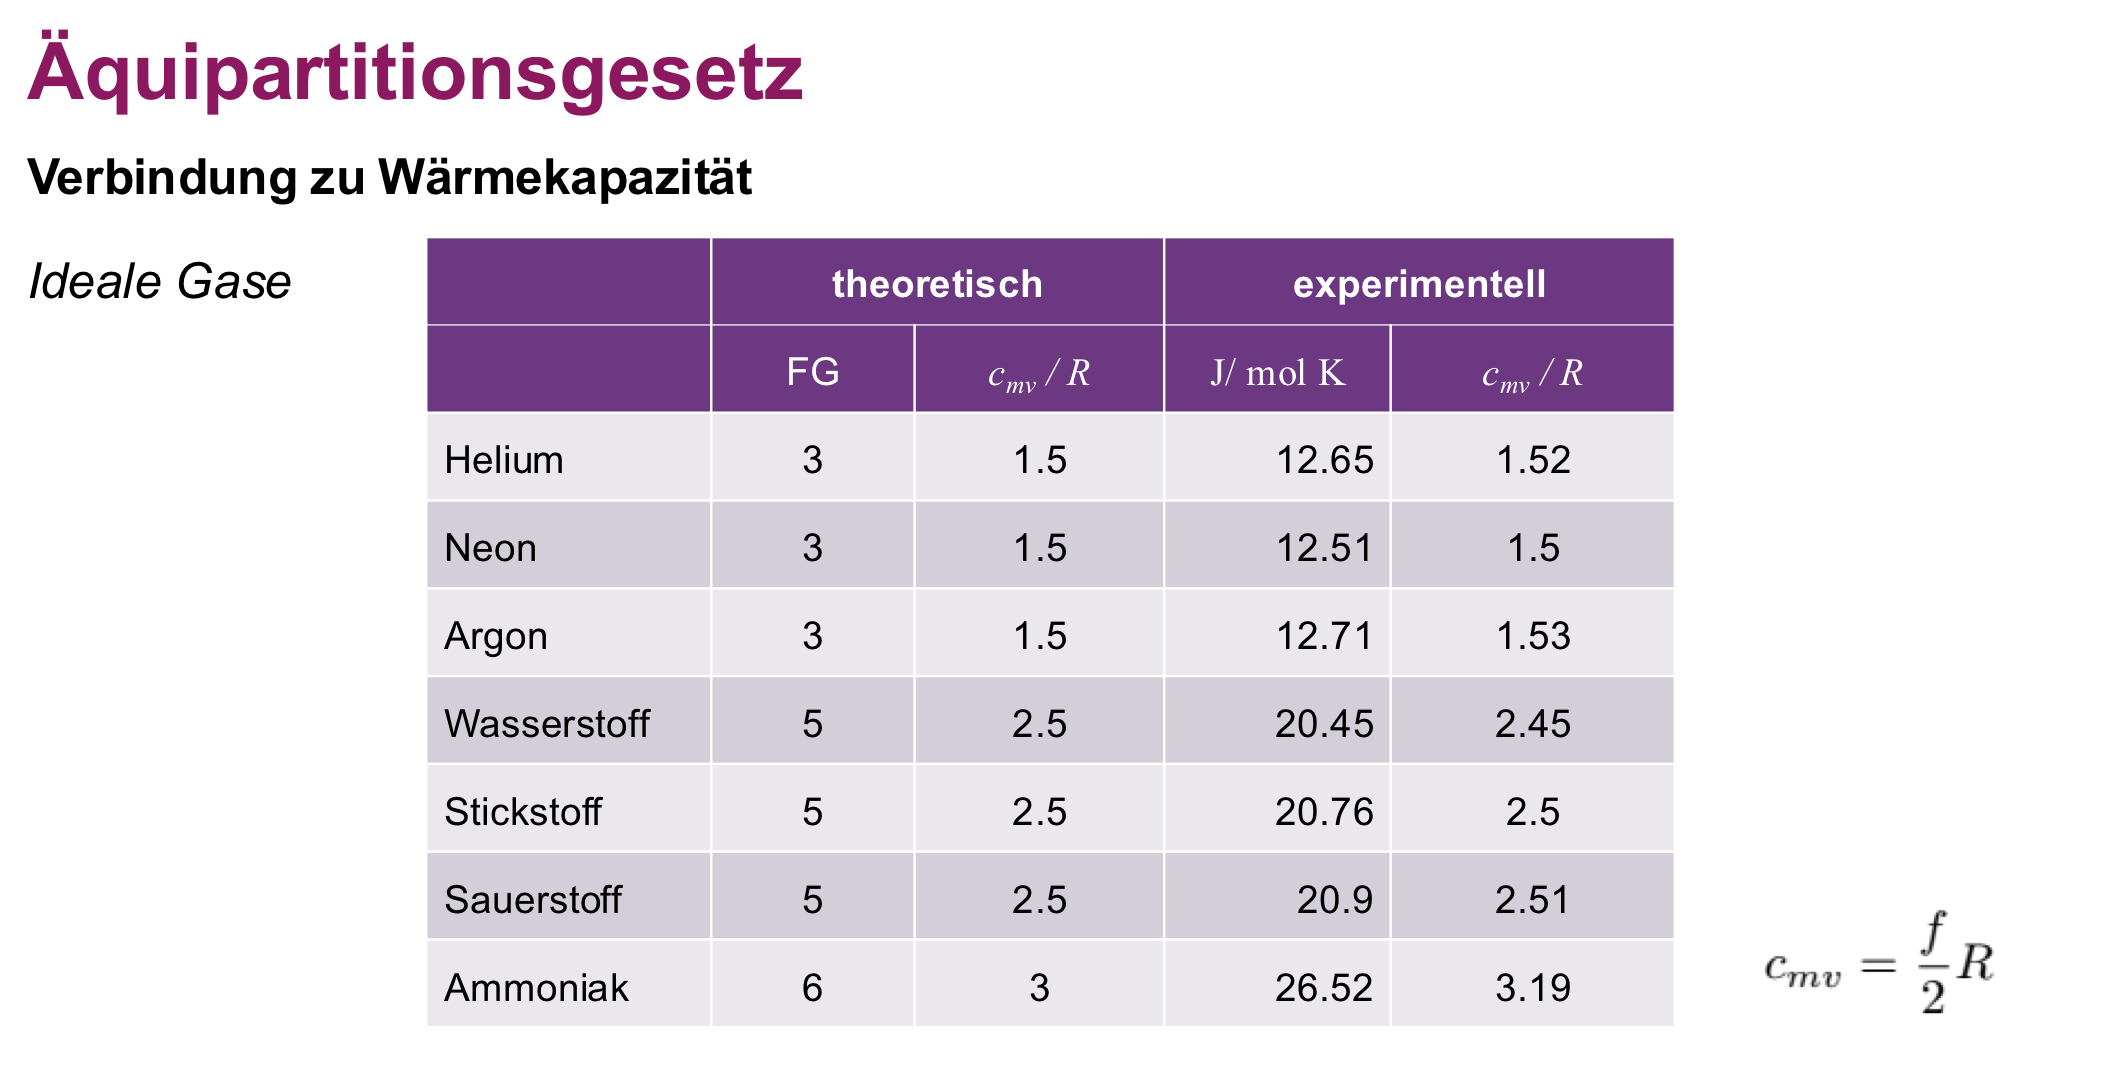
\includegraphics[width=0.9\columnwidth]{images/Ideale-Gase.PNG}
\end{center}

\subsubsection{Thermische Ausdehnung von Gasen}

\begin{itemize}
	\item Ausdehnung von Gasen ist sehr gross
	\item Bei \textbf{allen} Gasen ist die Ausdehnung \textbf{gleich}
	\item Volumen beim Nullpunkt ist \textbf{Null} 
\end{itemize}

\subsection{Phänomene von idealen Gasen}

\subsubsection{Annomalie des Wassers}

Die feste Form (Eis) ist leichter als die flüssige Form (Wasser) \\
Die \textbf{grösste Dichte weist Wasser bei 4 °C} auf, nicht beim Gefrierpunkt von $0 \, \celsius$

\smallskip

\textrightarrow\ Ein See gefriert somit nur an der Oberfläche. Am Grund des Sees beträgt die Wassertemperatur $4 \, \celsius$ 

\subsection{Phasen}

\begin{description}
	\item[Fest:] feste Gestalt; festes Volumen
	\item[Flüssig:] keine feste Gestalt; festes Volumen
	\item[Gasförmig:] keine feste Gesalt; kein festes Volumen
	\item[Plasma:] bei sehr hoher Temperatur ist Materie ionisiert (Elektronengas)
\end{description}


\subsubsection[Dampfdruck]{Dampfdruck $\boldsymbol{p_s(T)}$}

\begin{itemize}
	\item \textbf{Der Dampfdruck bedeutet das Gleichgewicht der Flüssigkeit mit ihrer Dampfphase}
	\item Der Dampfdruck ist das Niveau des kontanten Drucks im 2-Phasengebiet eines realen Gases nach van der Waals
	\item Der Dampfdruck ist nur \textbf{temperaturabhängig}
	\item Bei Kompression oder Expansion ändert sich der Dampfdruck nicht, sondern der Anteil Flüssigkeit zu Gas muss ändern
\end{itemize}

\begin{center}
	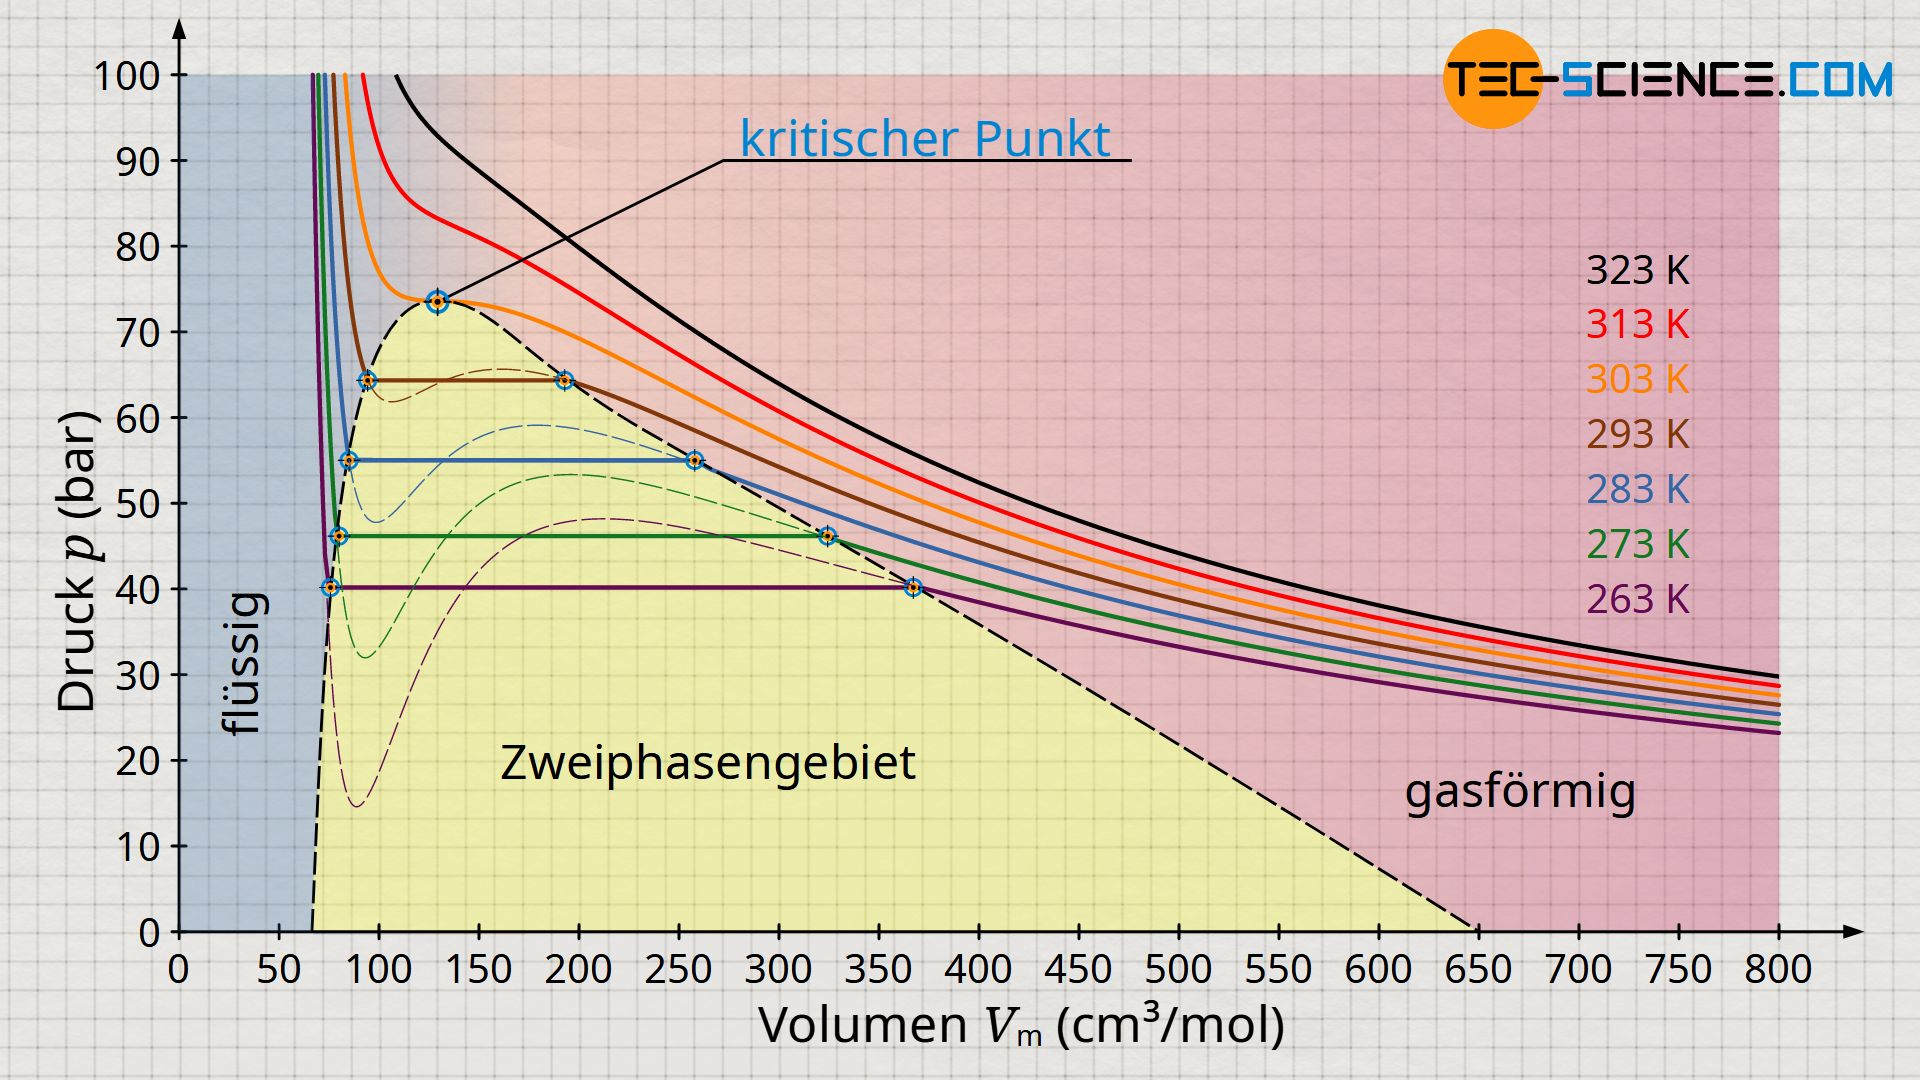
\includegraphics[width=0.9\columnwidth]{images/dampfdruck.jpg}
\end{center}

\begin{itemize}
	\item \textbf{Verdunsten} \textrightarrow\ Schnellste Teilchen treten aus Flüssigkeit aus
	\item \textbf{Sieden/Verdampfen} \textrightarrow\ Dampfdruck = Umgebungsdruck
\end{itemize}


\subsection{Temperatur}
\begin{itemize}
	\item Wärmestahlung = Berührungslose Übertragung von Wärme 
	\item In Form von elektromagnetischen Wellen ($\lambda$ @ IR)
	\item Körper absorbiert elektromagn. Strahlung und erhöht seine Temperatur
	\item Jeder Körper mit $T > 0 \, \kelvin$ straht Wärme ab (Temp-strahlung)
	\item Für jede Wellenlänge muss ein Körper gleich viel Energie abstahlen, wie er zuvor aufgenommen hat!
\end{itemize}
\smallskip

\subsection{Strahlungs-Gesetze - Strahlung} \label{subsec:Strahlung}

\subsubsection{Stefan-Boltzmann-Gesetz}

\begin{itemize}
	\item Idealer schwarzer Körper (Hohlraum) absorbiert \textbf{alle Wellenlängen zu 100 \%}
	\item Je mehr ein Körper absorbiert, desto mehr muss er emmitieren \textbf{(Energie-Gleichgewicht)}
\end{itemize}


Ein schwarzer Körper (=Hohlraumstrahler) der Temperatur $T$ hat eine totale Abstrahlungs-Leistung \textbf{pro Oberfläche} $K_S$ von: 
$$ \boxed{ K_S = \sigma \cdot T^4 }  $$


\renewcommand{\arraystretch}{1.3}
\begin{tabular}{c l c}
	$K_S$ 		& Schwarzkörper-Emission 																			& $[K_S] = \mathrm{\frac{W}{m^2}}$ 					\\
	$\sigma$ 	& Stefan-Boltzmann-Konstante $\sigma = 5.671 \cdot 10^{-8} \, \frac{\watt}{\meter^2 \, \kelvin^4}$ 	& $[\sigma] = \frac{\watt}{\meter^2 \, \kelvin^4}$	\\
	$T$ 		& \textbf{Absolute} Temperatur 																		& $[T] = \mathrm{K}$
\end{tabular}
\renewcommand{\arraystretch}{1}


\subsubsection{Wien'sches Verschiebungsgesetz}

Verschiebung der maximalen Wellenlänge:

$$ \boxed{ \lambda_{\rm max} \cdot T = \const = b } $$

\begin{tabular}{c l c}
	$\lambda_{\rm max}$	& Wellenlängen-Maximum (Planck) 							& $[\lambda_{\rm max}] = \meter$	\\
	$T$ 				& \textbf{Absolute} Temperatur 								& $[T] = \mathrm{K}$				\\
	$b$					& Konstante: $b = 2.898 \cdot 10^{-3} \, \meter \, \kelvin$	& $ [b] = \meter \, \kelvin$
\end{tabular}

\subsubsection{Planck'sches Gesetz der Quantenmechanik}

Ein Oszillator, welcher auf ein anderes Energieniveau (=Elektronen-Kreisbahnen nach Bohr) wechselt, setzt die Energiedifferenz 
$\Delta E$ in ein Lichtquant (Photon) mit entsprechender Frequenz $f$ um. \\
Je nach Vorzeichen von $\Delta E$ wird das Photon emmitiert oder absorbiert.

$$ \boxed { \Delta E = h \cdot f }  $$

\begin{tabular}{c l c}
	$\Delta E$ 	& spektrale Abstrahlung (Energie) 												& $[\Delta E] = \joule$ 				\\
	$h$ 		& Panck'sches Wirkungsquantum $h = 6.628 \cdot 10^{-34} \, \joule \, \second$	& $[h] =  \joule \, \second$			\\
	$f$ 		& Frequenz des Photons 															& $ [f] = \frac{1}{\second} = \hertz$
\end{tabular}


\pagebreak


\section{Anwendungsbeispiele}

\subsection{Viskosimeter}

\begin{center}
	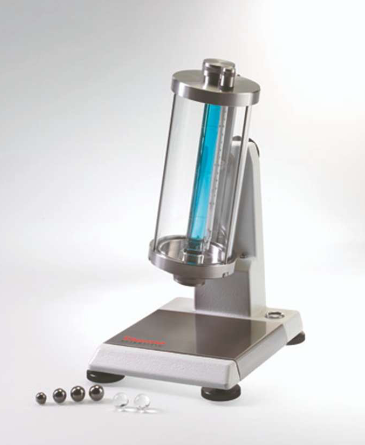
\includegraphics[scale = 0.5]{images/Viskosimeter.png}
\end{center}

\subsection{cw Werte}

\begin{center}
	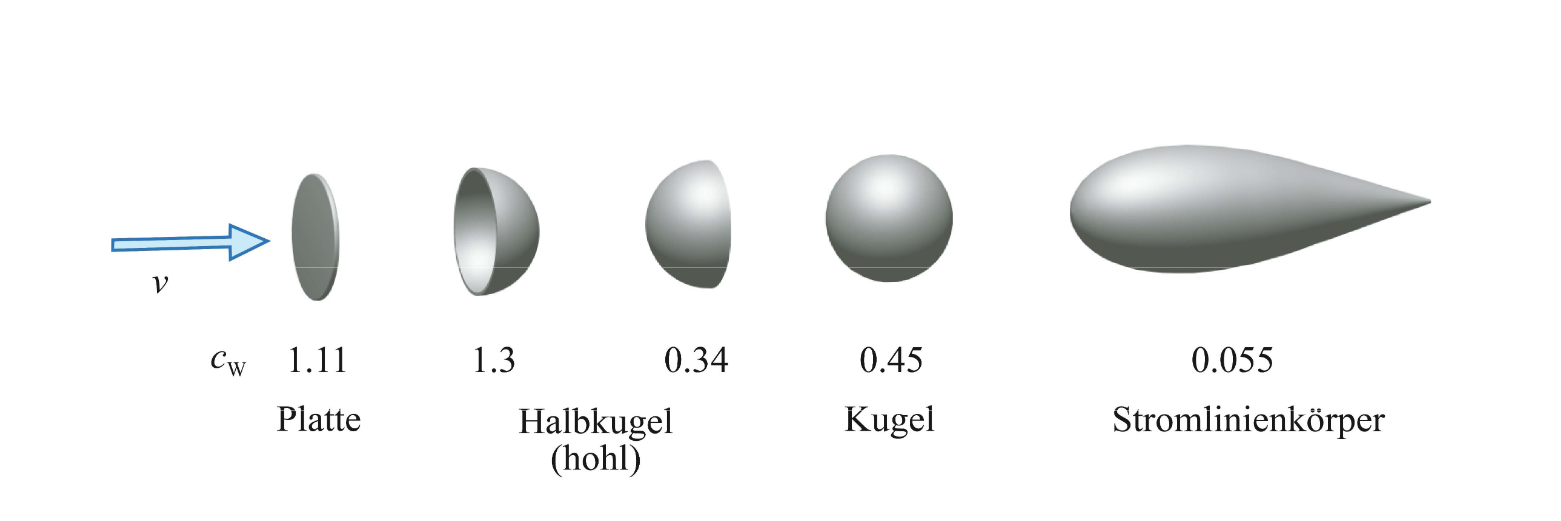
\includegraphics[scale = 0.2]{images/cw_werte.png}
\end{center}

\subsection{Toricelli beispiel}
\begin{tabular} {l l}
Ein Wasserbehälter ist 2 m hoch, unten ist ein kleines Loch  &  \\
daher gilt:& $v = \sqrt{2 \cdot g \cdot h}$  \\
eingesetzt: & $v = \sqrt{2 \cdot 9.81 \cdot 2}$  \\
\end{tabular}

\subsection{Barometer}

\begin{minipage}[t]{0.4\columnwidth}
	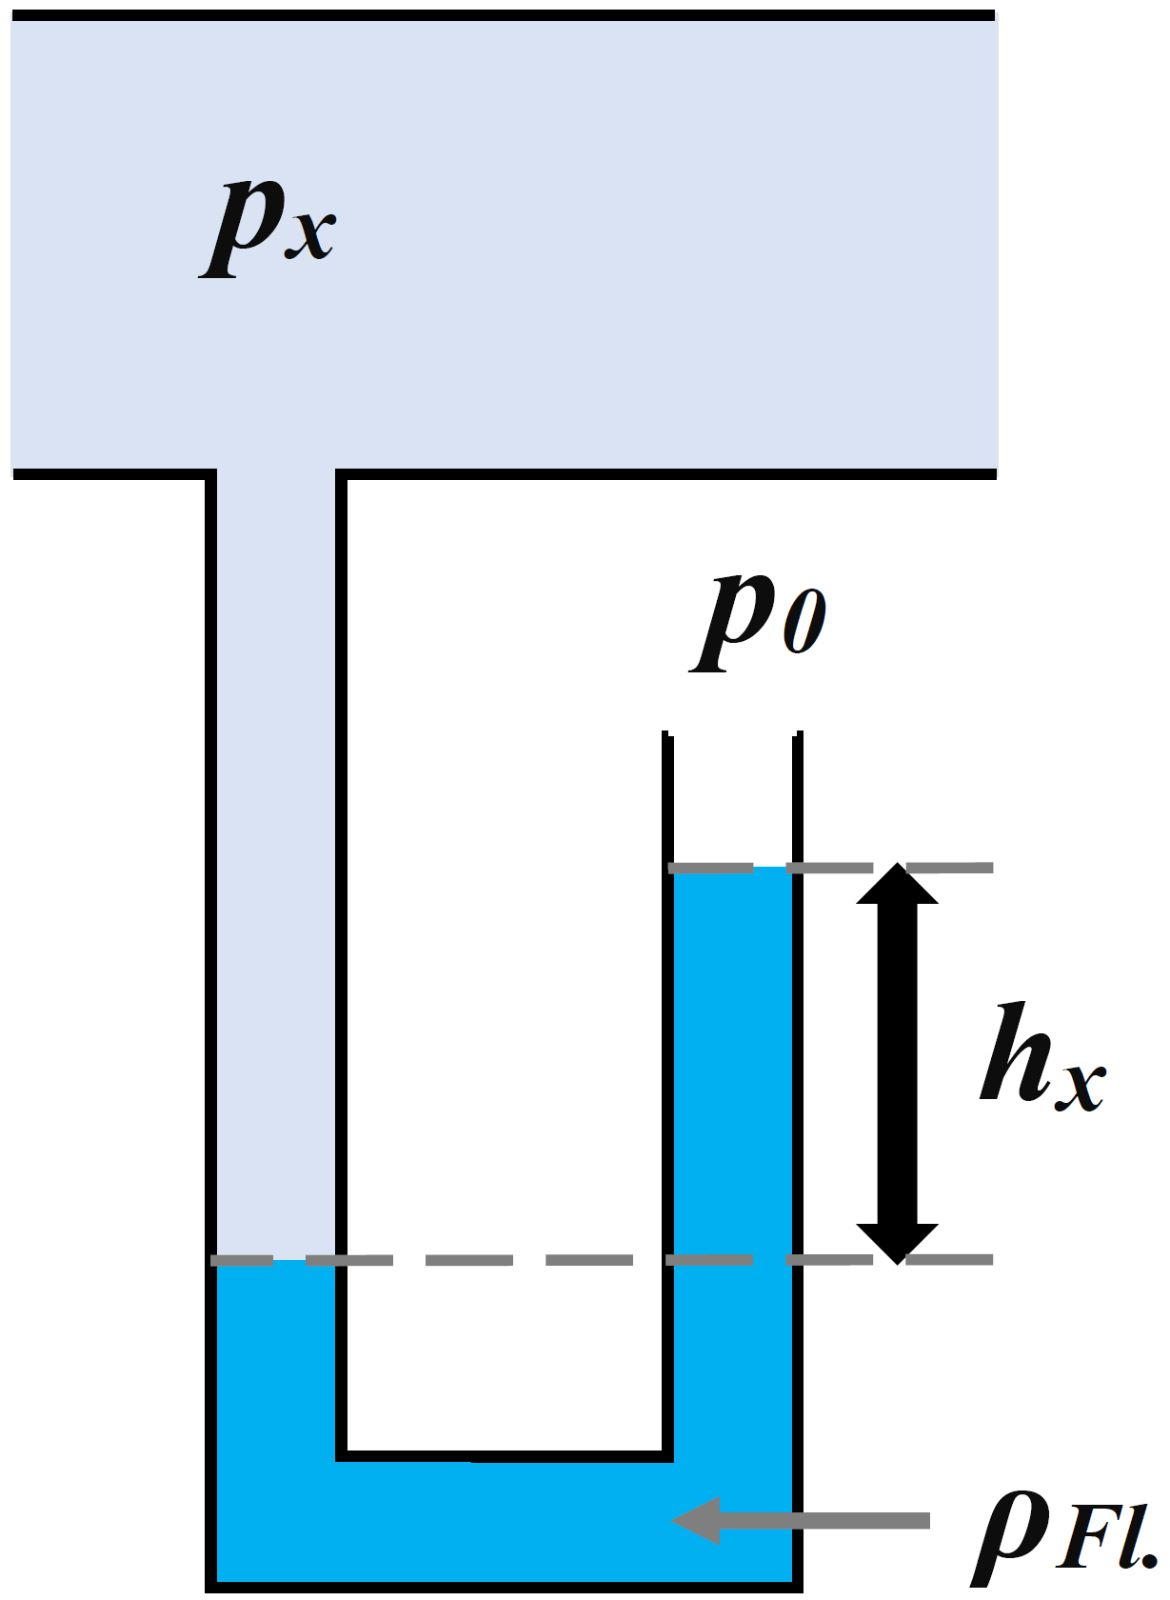
\includegraphics[width=\columnwidth, align=t]{images/manometer.jpg}
\end{minipage}
\hfill
\begin{minipage}[t]{0.5\columnwidth}
	$$ \boxed{ p_1 = p_0 + \underbrace{ \rho_{Fl} \cdot g \cdot h}_{\substack{p_s}} } $$
	
	\begin{tabular}{ll}
		$p_1$   & Gemessener Druck  \\
		$p_0$   & Luftdruck         \\
		$p_s$   & Schweredruck
	\end{tabular}
	
	\medskip
	
	\textrightarrow\ Bernoulli \\
	\textrightarrow\ Kontinuität
\end{minipage}


\subsection{Pitotrohr}
Prandtl'sches Staurohr; Staudruckmesser \\
Zur Messung von Strümungsgeschwindigkeiten 

\begin{center}
    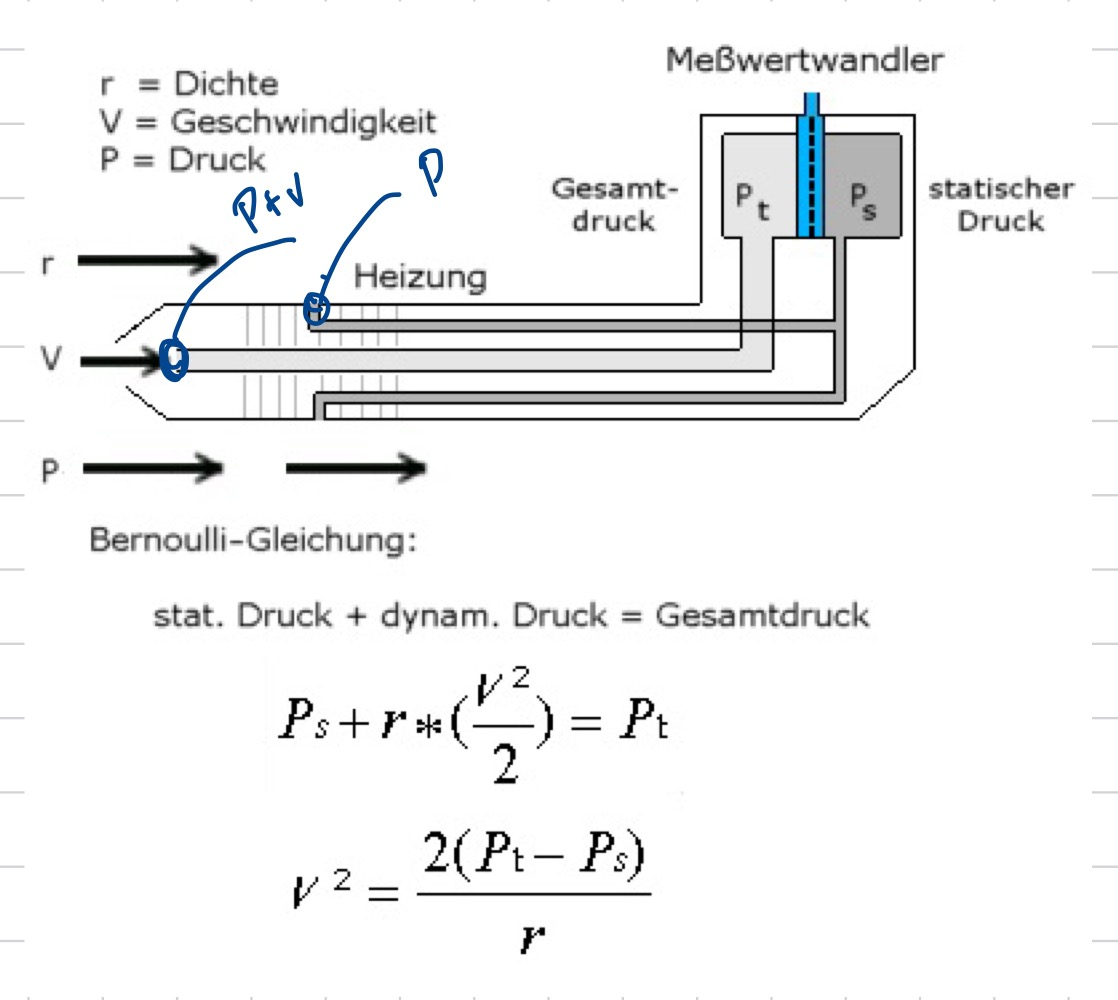
\includegraphics[width=0.73\columnwidth]{images/pitotrohr1.JPEG}
\end{center}


$$ \boxed{ \text{Bernoulli horizontal:} \quad \underbrace{p_1}_{\substack{p_L}} + \frac{1}{2} \, \rho_1 \cdot \underbrace{v_1^2}_{\substack{0}} = \underbrace{p_2}_{\substack{p_L - \Delta p}} + \frac{1}{2} \, \underbrace{\rho_2}_{\substack{\rho_L}} \cdot v_2^2} $$

$$ 0 = - \Delta p + \frac{1}{2} \, \rho_L \cdot v_2^2 \qquad \Rightarrow \Delta p =\frac{1}{2} \, \rho_L \cdot v_2^2 $$

$$ \text{Gleichsetzen:} \quad \Delta p = \rho_{Fl} \cdot g \cdot h $$


\subsection{Pumpe}

\vspace{-0.2cm}

$$ \boxed{ W = P \cdot t = F \cdot \Delta s = p \cdot A \cdot \Delta s = p \cdot \Delta V } \qquad  \qquad \boxed{ F = p \cdot A }  $$

$$ \boxed{ P =  \frac{W}{t} = \frac{p \cdot V}{t} = p  \cdot  \dot{V} } $$


\subsection{Bewegungen}

\vspace{-0.2cm}

$$ \boxed{ P = F \cdot v } \qquad \qquad \boxed{ E_{\rm kin} = \frac{1}{2} \, m \cdot v^2 } $$



\subsection{U-Rohr}

\begin{minipage}[t]{0.35\columnwidth}
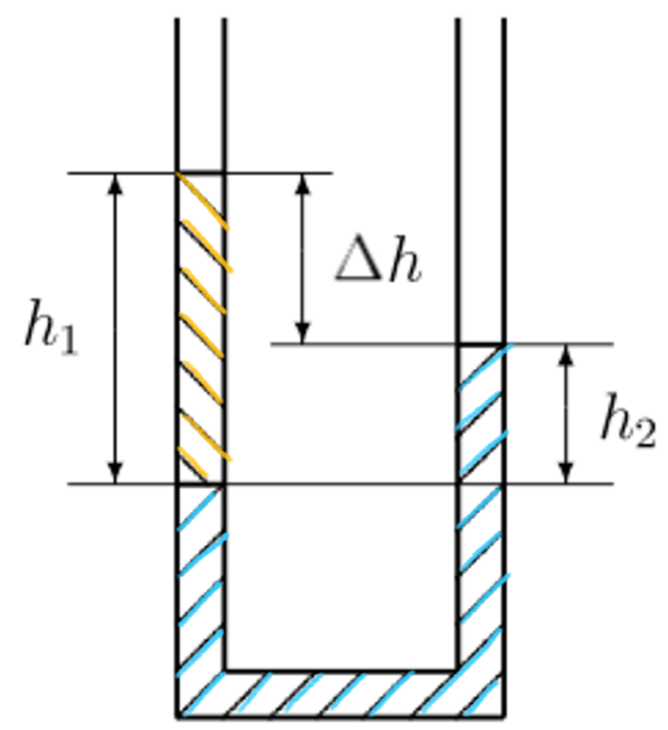
\includegraphics[width=\columnwidth, align=t]{images/u-rohr.png}
\end{minipage}
\hfill
\begin{minipage}[t]{0.6\columnwidth}

    Ansatz: Druckgleichgewicht 

    $$ \boxed{ p_1 = p_2 } $$

    $$ \boxed{ \rho_1 \cdot g \cdot h_1 = \rho_2 \cdot g \cdot h_2 } $$
\end{minipage}


\subsection{Wasser mit Dampf erhitzen}\label{subsec:Dampf}

Ein Tasse mit $m_W = 200 \, \gram$ Wasser  mit einer Temperatur von $T_K = 20 \, \celsius$ wird an
der Wasserdampfdüse einer Kaffeemaschine mittels Wasserdampf erhitzt. \\
Der aus der Kaffeemaschine ausströmende Wasserdampf ist $T_H = 96 \, \celsius$ heiss. \\
Am Schluss haben Sie 10 \% mehr Wasser in der Tasse. (entspricht $m_D$)\\
Wie warm ist das Wasser nun?

$$ \text{Ansatz: 1. Hauptsatz} \quad Q_{\rm zu} = Q_{\rm ab} $$ 

$$ m_W \cdot c_W \, (T_M - T_K) = q_s \cdot m_D + m_D \cdot c_W \, (T_H - T_M) $$


\subsection{Eis in Wasser schmelzen}

In einem Gefäss beifinden sich $m_W = 1 \, \kilogram$ Wasser. \\
Dazu wird ein Eiswürfel von $m_E = 20 \, \gram$ gegeben. \\
Das Eis hat eine Temperatur von $T_E = -5 \, \celsius$ und das Wasser hat eine Temperatur $T_W$. Die Temperatur $T_0$ steht 
für $0 \, \celsius$ bzw. $273.15 \, \kelvin$ \\
Gesucht ist die Mischtemperatur $T_M$ 

$$ \Delta Q_{\rm ab} = \Delta Q_{\rm zu} $$
$$ c_W \cdot m_W \cdot (T_W - T_M) = c_E \cdot m_E \cdot (T_0 - T_E) + q_f \cdot m_E + c_W \cdot m_E \cdot (T_M - T_0) $$


